\documentclass[onlytextwidth, aspectratio=169]{beamer}
\documentclass[onlytextwidth, aspectratio=169]{beamer}
\usepackage[utf8]{inputenc}
\usepackage{microtype}
\usepackage{amsmath}
\usepackage{amssymb}
\usepackage[nomessages]{fp} %\FPeval{\var-name}{2*sin(pi/6)}
\usepackage{siunitx} %units in math. eg 20\milli\meter
\usepackage{yhmath} % for arcs, overparenth command
\usepackage{tikz} %graphics
\usetikzlibrary{quotes, angles, arrows, arrows.meta}
%\usepackage{graphicx} already loaded by beamer class
%consider setting \graphicspath{{images/}}
%\parskip ?? to avoid paragraph indent
\usepackage{multicol} %may not need this package, just columns environment
\usepackage{venndiagram}

\subtitle[BECA]{Bronx Early College Academy}
\author[Huson]{Christopher J. Huson PhD}

\setbeamertemplate{headline}{\vskip2mm 
  \, BECA / \insertshortauthor \, / \inserttitle
  \hfill 
  \insertsection
  }

%Tick mark commands
\newcommand\ticks{}
  \def\ticks{{Bar[scale=2]}-{Bar[scale=2]}}
\newcommand\paraticks{}
  \def\paraticks{{Straight Barb[reversed, scale=2]}-{Straight Barb[scale=2]}}

\title{Geometry Unit 8: Year-to-date Regents review}
\date{13 February 2023 - 10 March 2023}

\begin{document}
\frame{\titlepage}
\section[Outline]{}
\frame{\tableofcontents}

\section{8.1 Triangle angles \hfill 13 February \,}
\begin{frame}{Learning Target: I can calculate triangle angles}
  {HSG.CO.C.10 Theorems about triangles \hfill \alert{8.1 Monday 13 February}}
  \begin{columns}
    \column{0.6\textwidth}
    Do Now
    \begin{enumerate}
      \item Review your Jumprope grades
      \item Right $\triangle ABC$ with m$\angle A = 53^\circ$. Find  m$\angle B$
    \end{enumerate}
    Lesson: Internal and external triangle angle measures \\
    Homework: Complete the classwork practice, Deltamath problem set
    \column{0.4\textwidth}
    \begin{flushright}
      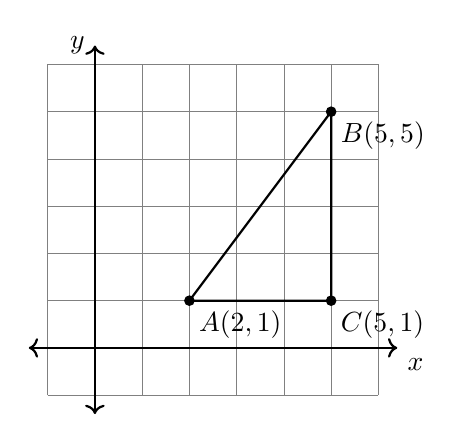
\begin{tikzpicture}[scale=0.6]
        \draw[help lines] (-1,-1) grid (6,6);
        \draw[thick, <->] (-1.4,0) -- (6.4,0) node [below right] {$x$};
        \draw[thick, <->] (0,-1.4)--(0,6.4) node [left] {$y$};
        \draw[thick] (2,1)--(5,5)--(5,1)--cycle;
        \draw [fill] (2,1) circle [radius=0.1] node[below right] {$A(2,1)$};
        \draw [fill] (5,5) circle [radius=0.1] node[below right] {$B(5,5)$};
        \draw [fill] (5,1) circle [radius=0.1] node[below right] {$C(5,1)$};
      \end{tikzpicture}
    \end{flushright}
  \end{columns}
\end{frame}

\begin{frame}{Triangle angle theorems, internal and external angle measures}
  {Find this information in your notebook (~October 24th)}
  \begin{columns}
    \column{0.6\textwidth}
      \begin{description}
        \item[Triangle sum theorem] m$\angle A + \text{m}\angle B + \text{m}\angle C = 180^\circ$
        \item[External angle theorem] m$\angle A + \text{m}\angle B = \text{m}\angle BCD$
        \item[Linear pair] angles that make a straight line, $180^\circ$
        \item[Supplementary] angles that sum to $180^\circ$
        \item[Complementary] angles that sum to $90^\circ$
        \item[Interior] Inside, internal
        \item[Exterior] Outside, external
      \end{description}
    \column{0.4\textwidth}
    \begin{flushright}
      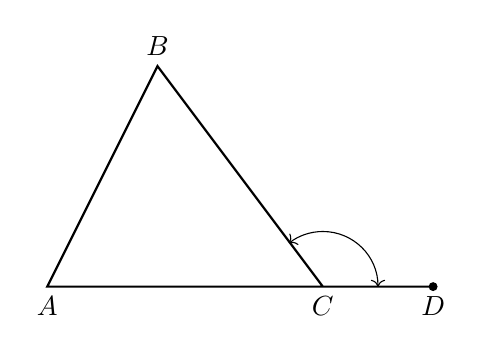
\begin{tikzpicture}[scale=0.7]
        \draw [thick]
        (9,0)node[below]{$D$}--
        (2,0)node[below]{$A$}--
        (4,4)node[above]{$B$}--
        (7,0)node[below]{$C$};
        \draw [fill] (9,0) circle [radius=0.07];
        \draw[<->] (8,0) arc (0:128:1);
        %\node at (2.8,0.4){$52^\circ$};
        %\node at (4.1,3.1){$48^\circ$};
      \end{tikzpicture}
    \end{flushright}
  \end{columns}
\end{frame}

\section{8.2 Transversals and isosceles triangles \hfill 14 February \,}
\begin{frame}{Learning Target: I can work with parallel lines}
  {HSG.CO.A.5 Congruence transformations \hfill \alert{8.2 Tuesday 14 February}}
  \begin{columns}
    \column{0.65\textwidth}
    Do Now: Isosceles $\triangle ABC$ has two angles measuring $65^\circ$. Find the measure of the 3rd angle, m$\angle C$.\\[0.5cm]
    Lesson: Isosceles triangles, parallel lines and transversals \\
    Homework: Complete classwork, Deltamath assignment
    \column{0.35\textwidth}
    \begin{flushright}
      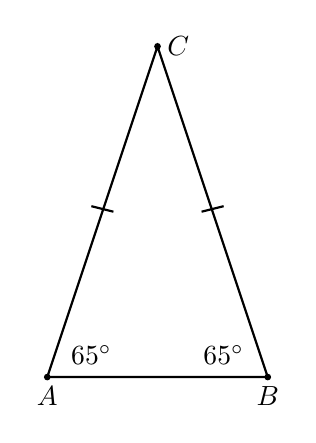
\begin{tikzpicture}[scale=0.7]
        \draw [thick](0,0)--(4,0)--(2,6)--(0,0);
        \draw [fill] (0,0) circle [radius=0.05] node[below]{$A$};
        \draw [fill] (4,0) circle [radius=0.05] node[below]{$B$};
        \draw [fill] (2,6) circle [radius=0.05] node[right]{$C$};
        \draw [thick] (0.8,3.1)--(1.2,3); %tick mark
        \draw [thick] (2.8,3)--(3.2,3.1); %tick mark
        \node at (0.8,0.4){$65^\circ$};
        \node at (3.2,0.4){$65^\circ$};
      \end{tikzpicture}
    \end{flushright}
  \end{columns}
\end{frame}

\begin{frame}{Isosceles base theorem: Sides $\cong$ \emph{iff} angles $\cong$}
  \begin{columns}
    \column{0.65\textwidth}
    Isosceles $\triangle ABC$ has two angles measuring $65^\circ$. Find the measure of the 3rd angle, m$\angle C$.\\[0.5cm]
    $65^\circ+65^\circ+x=180^\circ$ \\
    $130^\circ+x=90^\circ$ \\
    $x=30^\circ$
    \column{0.35\textwidth}
    \begin{flushright}
      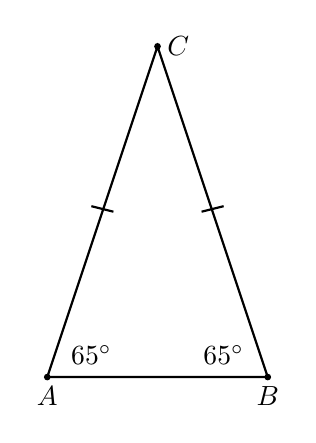
\begin{tikzpicture}[scale=0.7]
        \draw [thick](0,0)--(4,0)--(2,6)--(0,0);
        \draw [fill] (0,0) circle [radius=0.05] node[below]{$A$};
        \draw [fill] (4,0) circle [radius=0.05] node[below]{$B$};
        \draw [fill] (2,6) circle [radius=0.05] node[right]{$C$};
        \draw [thick] (0.8,3.1)--(1.2,3); %tick mark
        \draw [thick] (2.8,3)--(3.2,3.1); %tick mark
        \node at (0.8,0.4){$65^\circ$};
        \node at (3.2,0.4){$65^\circ$};
      \end{tikzpicture}
    \end{flushright}
  \end{columns}
\end{frame}

\begin{frame}{Two parallel lines and a transversal intersecting them}
  \begin{columns}
    \column{0.7\textwidth}
      \begin{description}
        \item[Vertical angles] at intersections, opposite angles are $\cong$ \vspace{0.5cm}
        \item[Corresponding angles] are congruent ($\angle 2 \cong \angle 6$)
        \item[Alternate interior] angles inside parallels, not on the same side, are congruent ($\angle 3 \cong \angle 6$)
        \item[Same side exterior] angles outside the transversal, on the same side, are supplementary (m$\angle 1 + \text{m}\angle 7 = 180^\circ$)
      \end{description}
    \column{0.3\textwidth}
    \begin{flushright}
      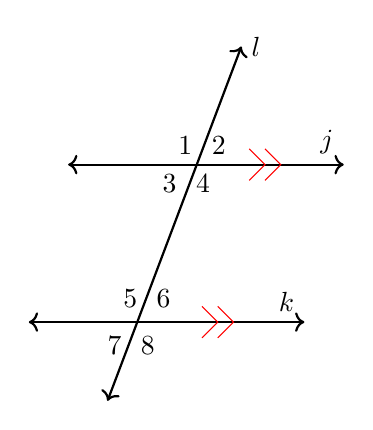
\begin{tikzpicture}[scale=1]
        \draw[<->, thick] (3.5,2)--(7,2)node[above left]{$j$};
        \draw[<->, thick] (3,0)--(6.5,0)node[above left]{$k$};
        \draw[<->, thick] (4,-1)--(5.7,3.5)node[right]{$l$};
        \draw[red] (5.2,-0.2)--(5.4,0)--(5.2,0.2);
        \draw[red] (5.4,-0.2)--(5.6,0)--(5.4,0.2);
        \draw[red] (5.8,1.8)--(6,2)--(5.8,2.2);
        \draw[red] (6,1.8)--(6.2,2)--(6,2.2);
        \node at (4.5,0.3) [left]{$5$};
        \node at (4.5,0.3) [right]{$6$};
        \node at (4.3,-0.3) [left]{$7$};
        \node at (4.3,-0.3) [right]{$8$};
        \node at (5.2,2) [above left]{$1$};
        \node at (5.2,2) [above right]{$2$};
        \node at (5,2) [below left]{$3$};
        \node at (5,2) [below right]{$4$};
      \end{tikzpicture}
    \end{flushright}
  \end{columns}
\end{frame}

\section{8.3 Midpoint, segment partition \hfill 16 February \,}
\begin{frame}{Learning Target: I can partition a line segment}
  {HSG.GPE.B.6 Partition a segment in a given ratio \hfill \alert{8.3 Thursday 16 February}}
  \begin{columns}
    \column{0.5\textwidth}
    Do Now: \\Given $T_{+a,+b}$ maps $(3,5) \rightarrow (9,8)$ \\
    Find $a$ and $b$ \\[0.5cm]
    Lesson: Ratios, partitioning a line segment \\
    Homework: Complete classwork, Deltamath assignment
    \column{0.4\textwidth}
    \begin{flushright}
      \begin{tikzpicture}[scale=0.5]
        \draw[thick, <->] (-1.4,0) -- (9.4,0) node [below right] {$x$};
        \draw[thick, <->] (0,-1.4)--(0,8.4) node [left] {$y$};
        \draw[thick, ->] (3,5)--(8.8,7.9);
        \draw [fill] (3,5) circle [radius=0.1] node[below right] {$A(3,5)$};
        \draw [fill] (9,8) circle [radius=0.1] node[above left] {$B(9,8)$};
      \end{tikzpicture}
    \end{flushright}
  \end{columns}
\end{frame}

\section{8.4 Area, volume, density, solids \hfill 27 February \,}
\begin{frame}{Learning Target: I can calculate area and volume}
  {HSG.GMD.A.3 Use volume formulas to solve problems \hfill \alert{8.4 Monday 27 February}}
  \begin{columns}
    \column{0.7\textwidth}
    Do Now: Find the volume of the box with dimensions: \\
    length = 5 cm \\
    width = 3 cm\\
    height = 10 cm \\[0.5cm]
    Lesson: Area, perimeter, volume, density, solids, cross sections \\
    Homework: Complete classwork, Deltamath assignment
    \column{0.3\textwidth}
    \begin{flushright}
      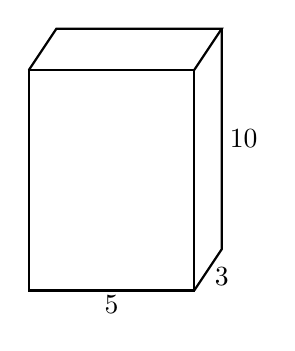
\begin{tikzpicture}[scale=0.7]
        \draw [-, thick] (0,0)--(3,0)--(3,4)--(0,4)--cycle;
        \draw [-, thick] (0,4)--(0.5,4.75)--(3.5,4.75)--(3,4);
        \draw [-, thick] (3,0)--(3.5,0.75)--(3.5,4.75);
        \node at (3.9, 2.75){$10$};
        \node at (1.5, -0.25){$5$};
        \node at (3.5, 0.25){$3$};
      \end{tikzpicture}
    \end{flushright}
  \end{columns}
\end{frame}

\begin{frame}{Use the Regents formula sheet or your notebook for formulas}
  $V_{cone}=\frac{1}{3}\pi r^2 h$
  \begin{columns}
    \column{0.5\textwidth}
    Given a cone with radius $r=6$ inches, volume $V=96 \pi$ cubic inches, and density $D=0.0267$ pounds per cubic inch
    \begin{enumerate}
      \item Solve for the height $h$ of the cone
      \item Find the \emph{slant height} $s$ using $a^2+b^2=c^2$
      \item Find the cone's weight $W$ to the \emph{nearest pound}
    \end{enumerate}
    \column{0.5\textwidth}
    \begin{flushright}
      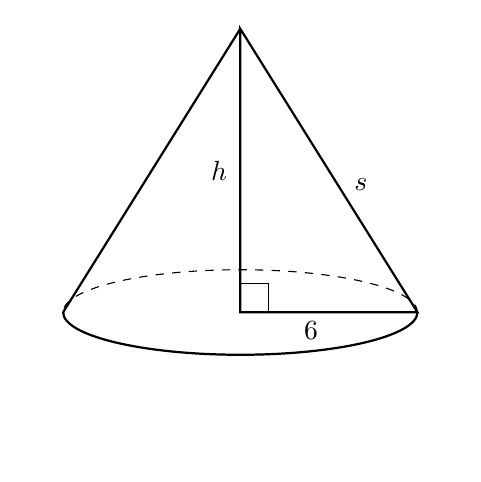
\begin{tikzpicture}[scale=0.9]
        \draw [thick] (0,0)--(2.5,0)--(0,4)--cycle;
        \draw (0,0)++(0.4,0)--++(0,0.4)--+(-0.4,0);
        \draw [thick] (0,4)--(-2.5,0);
        \node at (1,0)[below]{$6$};
        \node at (-0.3,2){$h$};
        \node at (1.7,1.8){$s$};
        \draw [dashed] (0,0) ellipse [x radius=2.5,y radius=0.6];
        \clip (-3,-2) rectangle (3,0);
        \draw [thick] (0,0) ellipse [x radius=2.5,y radius=0.6];
      \end{tikzpicture}
    \end{flushright}
  \end{columns}
  \begin{description}
    \item[slant height] The diagonal length of the side of a cone or pyramid
  \end{description}
\end{frame}

\begin{frame}{The study of 3-dimensional shapes are called solid geometry}
  \begin{columns}
    \column{0.6\textwidth}
    What 3-dimensional shape is made when a right triangle is rotated around its longer edge? \vspace{1cm}
    \begin{description}
      \item[cross section] the shape made by a plane intersecting a solid
    \end{description}
    \column{0.4\textwidth}
    \begin{flushright}
      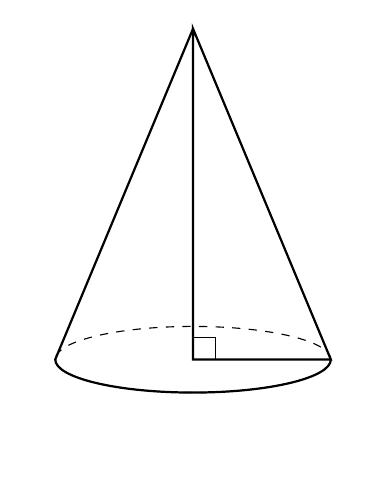
\begin{tikzpicture}[scale=0.7]
        \draw [thick] (0,0)--(2.5,0)--(0,6)--cycle;
        \draw (0,0)++(0.4,0)--++(0,0.4)--+(-0.4,0);
        \draw [thick] (0,6)--(-2.5,0);
        \draw [dashed] (0,0) ellipse [x radius=2.5,y radius=0.6];
        \clip (-3,-2) rectangle (3,0);
        \draw [thick] (0,0) ellipse [x radius=2.5,y radius=0.6];
      \end{tikzpicture}
    \end{flushright}
  \end{columns}
\end{frame}

\section{8.5 Analytic geometry graphing \hfill 3 March \,}
\begin{frame}{Learning Target: I can graph linear equations and systems}
  {HSA.REI.C.6 Solve systems of linear equations \hfill \alert{8.5 Friday 3 March}}
  \begin{columns}
    \column{0.6\textwidth}
    Do Now: Graph the line $y=\frac{1}{2}x+2$ \\[0.5cm]
    Lesson: slope-intercept form, systems \\
    Homework: Complete classwork, Deltamath assignment
    \column{0.4\textwidth}
    \begin{flushright}
      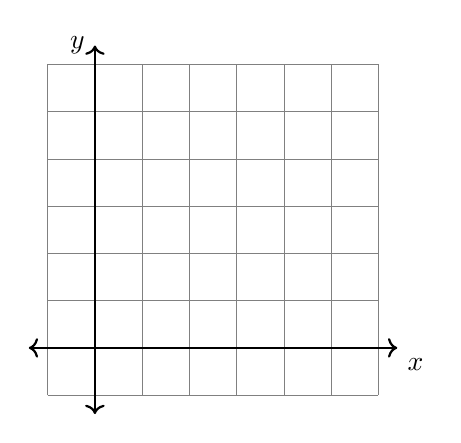
\begin{tikzpicture}[scale=0.6]
        \draw[help lines] (-1,-1) grid (6,6);
        \draw[thick, <->] (-1.4,0) -- (6.4,0) node [below right] {$x$};
        \draw[thick, <->] (0,-1.4)--(0,6.4) node [left] {$y$};
      \end{tikzpicture}
    \end{flushright}
  \end{columns}
\end{frame}

\begin{frame}{Solving a system using a graphing calculator}
  \begin{columns}
    \column{0.6\textwidth}
    $$f(x)=-\frac{1}{2}x+6$$
    $$g(x)=\frac{3}{4}x+1$$
      \onslide<2->{$f(4)=-\frac{1}{2}(4)+6=-2+6=4$ \\
      $g(4)=\frac{3}{4}(4)+1=3+6=4$}
    \onslide<1>{\begin{description}
      \item[system] two or more equations with the same variables
      \item[intersection] the point where two lines cross, or the $(x,y)$ values that satisfy both equations
    \end{description}}
    \column{0.4\textwidth}
    \begin{flushright}
      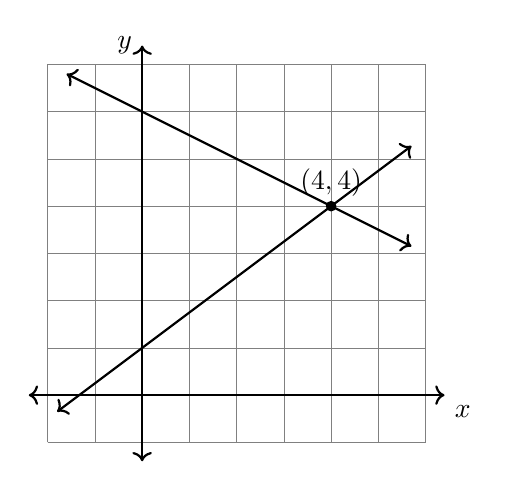
\begin{tikzpicture}[scale=0.6]
        \draw[help lines] (-2,-1) grid (6,7);
        \draw[thick, <->] (-2.4,0) -- (6.4,0) node [below right] {$x$};
        \draw[thick, <->] (0,-1.4)--(0,7.4) node [left] {$y$};
        \pause
          \draw[thick, <->,domain=-1.6:5.7] plot(\x,-0.5*\x+6);
          \draw[thick, <->,domain=-1.8:5.7] plot(\x,0.75*\x+1);
          \draw [fill] (4,4) circle [radius=0.1]node[above]{$(4,4)$};
      \end{tikzpicture}
    \end{flushright}
  \end{columns}
\end{frame}

\section{8.6 Analytic geometry slope applications \hfill 6 March \,}
\begin{frame}{Learning Target: I can use slope to solve problems}
  {HSG.GPE.B.5 Use slope to solve geometric problems \hfill \alert{8.6 Monday 6 March}}
  \begin{columns}
    \column{0.6\textwidth}
    Do Now: Solve the system in your graphing calculator: 
      $$f(x)=-x+2$$
      $$g(x)=-3x-2$$
    \onslide<1>{
      Lesson: Perpendicular and parallel slopes, applications \\
      Homework: Complete classwork, Deltamath assignment}
    \column{0.4\textwidth}
    \begin{flushright}
      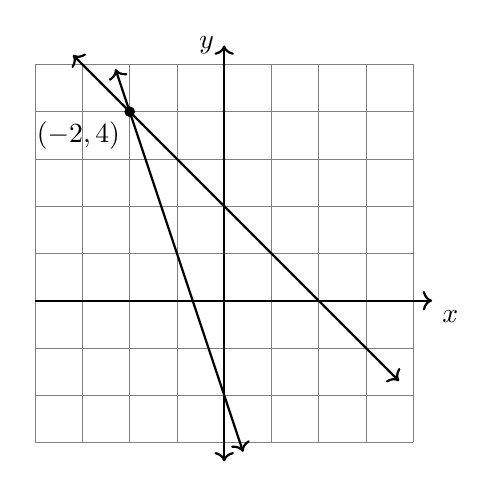
\begin{tikzpicture}[scale=0.6]
        \draw[help lines] (-4,-3) grid (4,5);
        \draw[thick, ->] (-4,0) -- (4.4,0) node [below right] {$x$};
        \draw[thick, <->] (0,-3.4)--(0,5.4) node [left] {$y$};
        \pause
          \draw[thick, <->,domain=-3.2:3.7] plot(\x,-\x+2);
          \draw[thick, <->,domain=-2.3:0.4] plot(\x,-3*\x-2);
          \draw [fill] (-2,4) circle [radius=0.1]node[below left]{$(-2,4)$};
      \end{tikzpicture}
    \end{flushright}
  \end{columns}
\end{frame}

\begin{frame}{Use slopes to prove special polygons}
  \begin{columns}
    \column{0.6\textwidth}
    Find each line's equation and their relationships
    \begin{enumerate}
      \item Find the equation of line $f$
      \item Find the equation of line $k$
      \item Show that $f \perp k$ because $m_f \times m_k = -1$
      \item Find and label the slopes of $g$ and $l$
      \item Show the polygon is a rectangle
    \end{enumerate}
    \column{0.4\textwidth}
    \begin{flushright}
      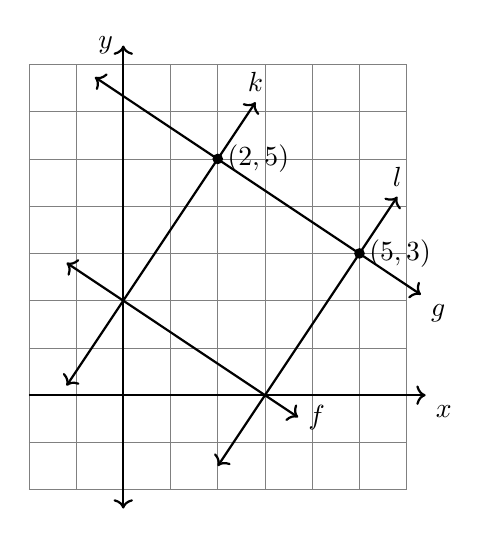
\begin{tikzpicture}[scale=0.6]
        \draw[help lines] (-2,-2) grid (6,7);
        \draw[thick, ->] (-2.0,0) -- (6.4,0) node [below right] {$x$};
        \draw[thick, <->] (0,-2.4)--(0,7.4) node [left] {$y$};
        \draw[thick, <->,domain=-1.2:3.7] plot(\x,-0.667*\x+2)node[right]{$f$};
        \draw[thick, <->,domain=-1.2:2.8] plot(\x,1.5*\x+2)node[above]{$k$};
        \draw[thick, <->,domain=-0.6:6.3] plot(\x,-0.667*\x+6.33)node[below right]{$g$};
        \draw[thick, <->,domain=2:5.8] plot(\x,1.5*\x-4.5)node[above]{$l$};
        \draw [fill] (2,5) circle [radius=0.1]node[right]{$(2,5)$};
        \draw [fill] (5,3) circle [radius=0.1]node[right]{$(5,3)$};
      \end{tikzpicture}
    \end{flushright}
  \end{columns}
\end{frame}

\section{8.7 Analytic geometry distance applications \hfill 7 March \,}
\begin{frame}{Learning Target: I can calculate distance in context}
  {HSG.GPE.B.7 Use coordinates to compute perimeters of polygons \hfill \alert{8.7 Tuesday 7 March}}
  \begin{columns}
    \column{0.6\textwidth}
    Do Now: Find the distance between the intercepts of the line show on the graph \\[0.5cm]
    Lesson: Distance formula, applications, simplifying radicals \\
    Homework: Complete classwork, Deltamath assignment \\[0.5cm]
    \alert{Unit test Friday}, Deltamath and problem sets due
    \column{0.4\textwidth}
    \begin{flushright}
      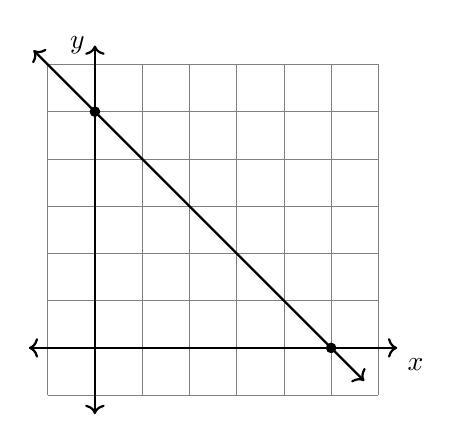
\begin{tikzpicture}[scale=0.6]
        \draw[help lines] (-1,-1) grid (6,6);
        \draw[thick, <->] (-1.4,0) -- (6.4,0) node [below right] {$x$};
        \draw[thick, <->] (0,-1.4)--(0,6.4) node [left] {$y$};
        \draw[thick, <->,domain=-1.3:5.7] plot(\x,-1*\x+5);
        \draw [fill] (5,0) circle [radius=0.1];
        \draw [fill] (0,5) circle [radius=0.1];
      \end{tikzpicture}
    \end{flushright}
  \end{columns}
\end{frame}

\begin{frame}{Use distance to prove special polygons}
  \begin{columns}
    \column{0.6\textwidth}
    Prove the quadrilateral is a rhombus
    \begin{enumerate}
      \item Apply the distance formula to each pair of points
      \item State the equality of the side lengths and the congruence of the sides
      \item State the conclusion, that the quadrilateral is a rhombus
    \end{enumerate}
    \column{0.4\textwidth}
    \begin{flushright}
      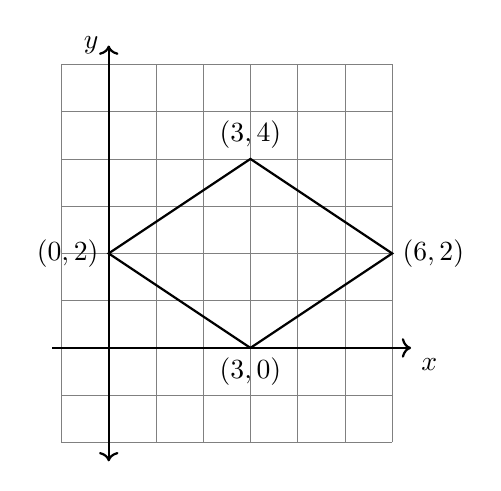
\begin{tikzpicture}[scale=0.6]
        \draw[help lines] (-1,-2) grid (6,6);
        \draw[thick, ->] (-1.2,0) -- (6.4,0) node [below right] {$x$};
        \draw[thick, <->] (0,-2.4)--(0,6.4) node [left] {$y$};
        \draw[thick] (0,2)node[left]{$(0,2)$}--
          (3,4)node[above]{$(3,4)$}--
          (6,2)node[right]{$(6,2)$}--
          (3,0)node[below]{$(3,0)$} -- cycle;
      \end{tikzpicture}
    \end{flushright}
  \end{columns}
\end{frame}

\section{8.8 Peer unit review \hfill 9 March \,}
\begin{frame}{Learning Target: I can use volume formulas to solve problems}
  {HSG.GMD.A.3 Use volume formulas to solve problems \hfill \alert{8.8 Thursday 9 March}}
    Do Now: Write in your notebook
    \begin{enumerate}
      \item Your strongest two skills in this unit
      \item Your weakest 2 topics (and why)
      \item Your current Jumprope grade
      \item Your goal for this trimester's report card grade in Geometry
    \end{enumerate} \bigskip
    Lesson: Unit review \\
    Notebook check, uniforms professionalism grade \\[0.5cm]
    \alert{Unit test tomorrow}, Deltamath and problem sets due
\end{frame}

\begin{frame}{Notebook check scoring}
  {Start quickly at the beginning of class: notebook, pencil, folder, calculator; get to work}
    Jumprope mastery score
    \begin{enumerate}
      \item I have a notebook $\rightarrow$ 1
      \item I have class notes $\rightarrow$ 2
      \item I have stars indicating I quickly sit down and write the learning target $\rightarrow$ 3
      \item I have stars and I complete the Do Now right away $\rightarrow$ 4
    \end{enumerate} \bigskip
\end{frame}

\end{document}